\chapter{Neural Networks and Backpropogation}

When dealing with increasingly complex data, it is not practical to deal with linear score functions with just a single weight matrix. These are usually of the form $f = Wx$. With a neural network, we can have a non-linear function that let's us obtain more complex decision boundaries.

3Blue1Brown videos are a great source to learn about Neural Networks. They are now the state of the art for machine learning and widely used for a variety of applications. From images to language processing, variations of neural networks are common. 

Neural networks are very powerful and perform a wide variety of tasks. They are universal function approximators. Now, contrasting with our previous linear function, we can imagine that a 2-layer Neural Network $f=W_2 max(0, W_1 x)$. Here $x \epsilon R^D$, $W_1 \epsilon R^{H\times D}$, $W_2 \epsilon R^{C \times H}$.

Similarly, for a 3-layer neural network, $f=W_3max(0, W_2max(0, W_1x))$. Visualizations of this can be seen in \href{http://cs231n.stanford.edu/slides/2020/lecture_4.pdf}{cs231n} slides.

\section{The Probability Explanation}

Neural networks essentially model the maximum likelihood estimate. Look at it this way: We have a set of parameters, that with our input give us an output. We want the output to be the best possible one (so for a classification problem, increase the probability of the correct class). Training a neural network does that! The best set of parameters is subsequently the maximum likelihood estimate. 

Why do we use negative log likelihood? Well, both are the same. Truly. They represent the same probabilistic distribution and the best values are the same. It's just that we negative log likehood because we want to minimize the loss function.

\section{Activation Functions}

There are various activation functions which are all non-linear. The previous equations used $max$ which is a non linear function. This is an example of an activation function ReLU. RELU is the most common activation function and widely used. Leaky-RELU is also used. The cs231n slides has a great list of possible activation functions. We don't tend to use sigmoid since it tends to kill gradients. Gradients will vanish and hence, can't be used for neural networks. It's the same thing for $tanh$.

\textit{For more on vanishing gradients in sigmoids and dying ReLUs, look at \href{https://medium.com/@karpathy/yes-you-should-understand-backprop-e2f06eab496b}{these notes by Andrej Karpathy}.}

This is also covered in some more depth in the "Training" section of the chapter.

\section{Architecture}

\begin{figure}[h]
    \centering
    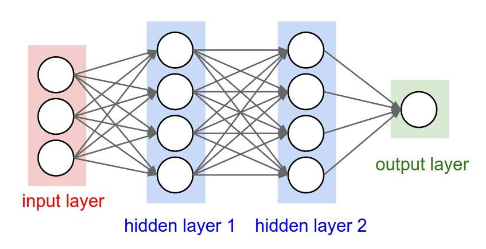
\includegraphics{img/Neural Network.png}
    \caption{Neural Network}
    \label{fig:neural-network}
\end{figure}

The neural network can be visualized to have an input layer - for its features, hidden layers (determined by the matrices in between), and an output layer. For a regression problem, the output layer would just be a single node but for a classification problem it would likely be the number of classes.

The "forward pass" refers to calculation process, values of the output layers from the inputs data. It's traversing through all neurons from first to last layer.

The loss function is calculated from the output values. 

And then "backward pass" refers to process of counting changes in weights (de facto learning), using gradient descent algorithm (or similar). Computation is made from last layer, backward to the first layer.

\textbf{Sidenote:} There is a problem with ReLU - dead neurons since gradient is 0 since ReLU is 0 when input is less than 0. Hence, leaky ReLU was created. However, ReLU has been found to be better in some instances.

There is only one cost function for a neural network - one for the entire network - not for each layer.

\section{Backpropogation}

In gradient descent, we calculated derivative/gradient and used that information to change our input. This was a gradual change and essentially decided by the change of the function with respect to the parameters. The same can be thought of for neural networks. The weights of each layer will determine the effectiveness of the network and hence, we need to set these weights appropriately. Unfortunately, it is not easy to calculate gradient manually. This is where the idea of backpropogation comes into the picture. 

"Backpropagation is for calculating the gradients efficiently, while optimizers is for training the neural network, using the gradients computed with backpropagation. In short, all backpropagation does for us is compute the gradients. Nothing more." from \href{https://mlfromscratch.com/neural-networks-explained/#/}{this.}

To understand the way this works pictorially, look at computation graphs in the \href{http://cs231n.stanford.edu/slides/2020/lecture_4.pdf}{cs231n slides}.

\href{http://neuralnetworksanddeeplearning.com/chap2.html}{This} is a very detailed source to understand backprogation. It is from a larger book about neural networks.

The way we might discover how to calculate gradients in the backpropagation algorithm is by thinking of this question:

\textit{How might we measure the change in the cost function in relation to a specific weight, bias or activation?}

\subsection{Intuition}

The 3Blue1Brown video explains backpropogation really well. Let us assume that we have just one example, and a neural network with a few hidden layers. Based on the weights and biases at these layers, we get an output vector with varying degrees of "activation". Now, each of these nodes will also have an ideal activation. For instance, our neural network may assign a score of 0.2 to a node, when ideally it is 1. How did we get this score? This score is the sum of the product of weights and the activation of the previous layer. So, we want to increase the activation of certain nodes in the previous layer and try increasing their importance as well - as long as they can help increase our output score. Vice versa, if our output score is higher than required, we want to reduce the values of weights and activation in previous layer. We can also bring about a change in the output by changing the bias. Note how we have identified the importance of the bias, and weights in some form. We see that there is a requirement to proportionally increase/decrease weights. This is just in regard to a single output node! Each output node will have connections to the previous layer and will also have some "requirements" about how much the weights should be tweaked. The idea is - if we satisfy the request of all these nodes, we are closer to a perfect solution. But is this the end? No.

The previous layer has now received some requests about how it should change. There may be other hidden layers though. Hence, we must recurse and move \textbf{backwards} through the network.

This was just for one training example! If we follow this routine and see what changes each example desires, and average it - it is essentially the negative gradient of the cost function.

\subsection{Simplified Math}

\href{https://www.youtube.com/watch?v=tIeHLnjs5U8}{A video by 3Blue1Brown} - obviously. Is very useful to understand what the gradients we are calculating represent. As mentioned earlier, calculating gradients manually is a pain.

In backpropogation, we measure the partial derivative of the cost function to weights, biases, and even the activation of previous layers.

Let us assume that we have a function such as $q = x + y$. This output $q$ is then fed to another function $f$ which is the final output of our computation graph. For ease refer to this example in figure \ref{fig:c_graph}.

\begin{figure}[t]
    \centering
    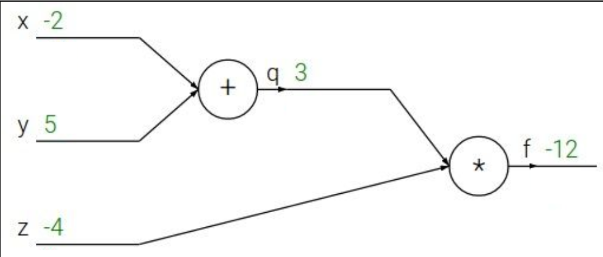
\includegraphics{img/computational-graph.png}
    \caption[width=5cm]{Computation Graph for Backprop Example}
    \label{fig:c_graph}
\end{figure}

Now, if we try to calculate the partial derivative of $f$ with respect to input $y$, we cannot directly compute it. We must use chain rule such that we get \[ \frac{\partial f}{\partial y} = \frac{\partial f}{\partial q} \frac{\partial q}{\partial y} \]
Here we refer to $\frac{\partial f}{\partial q}$ as the upstream gradient as it is a gradient that is not local to $y$ in some sense. The local gradient here is $\frac{\partial q}{\partial y}$. The product of these two may then be relevant as an upstream gradient for another partial derivative (assume that $y$ was also a function). Hence, with respect to this particular function, this is the downstream gradient.

\subsubsection{Patterns in gradient flow}
We observe that the addition operation is a \textit{gradient distributor}. This is because local gradient is 1.

The multiplication gate is a \textit{swap multiplier}. This is because local gradient is the other variable in the multiplication. Hence, we multiply the other input with the upstream gradient.

This is essentially what happens in backward pass. Obviously, note that the graph must be topologically sorted for us to calculate gradients properly since we constantly need an upstream gradient. Traversing in the reverse order of a topological sort will guarantee this.

\subsection{Real Math}

So far, we've done backpropogation with scalars (in the computational graph). But what about vector valued functions? - the type we'll be dealing with in neural networks.

Let us assume that we have $x \epsilon R^N$, and $y \epsilon R^M$ - they are both vectors. To see how for each element of $x$ changes, how $y$ changes requires vector derivatives - the Jacobian

I would write this part entirely but there is already an amazing resource for this - \href{https://github.com/RoboticsIIITH/summer-sessions-2020/blob/master/lecture-slides/deep_learning/backprop_linear_layer.pdf}{notes by Justin Johnson}. It describes how upstream gradients can be assumed to be give, and we need to calculate the local gradients. When we look at the dimensions, the local gradient is in fact a Jacobian. This matrix is so large that it often cannot even fit in memory! Hence, we are forced to compute the product of local and upstream gradient without explicitly calculating the Jacobian. The PDF describes this very well but in the end, we find that for a function such as $Y=XW$, then for $L$ - the loss function, 

\begin{equation}
    \frac{\partial L}{\partial X} = \frac{\partial L}{\partial Y} W^T
\end{equation}

Similarly, to calculate $\frac{\partial L}{\partial W}$ without the Jacobian $\frac{\partial Y}{\partial W}$ with:

\begin{equation}
    \frac{\partial L}{\partial W} = X^T \frac{\partial L}{\partial Y}
\end{equation}

This strategy of thinking one element at a time can help you to derive equations for backpropogation for a layer even when the inputs and outputs to the layer are tensors of arbitrary shape.

\subsubsection{Backprop for ReLU}

\begin{equation}
    \Big( \frac{\partial L}{\partial x} \Big)_{i} = \begin{cases}
       \Big(\frac{\partial L}{\partial z} \Big)_{i} &\quad\text{if} x_i > 0\\
       \text{0} &\quad\text{otherwise}\\
     \end{cases}
\end{equation}

\subsection{Micrograd}

Micrograd is a tiny autograd engine that let's us easily understand all the previous concepts of gradients. It is meant to understand how gradients are calculated, and how backward propagation works. \href{https://github.com/RoboticsIIITH/summer-sessions-2020/blob/master/lecture-slides/deep_learning/vector_derivatives.pdf}{These slides (at the end)} has some code snippets from the original \href{https://github.com/karpathy/micrograd}{repository}. It is worth looking at to get a rudimentary understanding of how pytorch works.

\section{Training}

The basic pipeline for training a neural network is:

\begin{enumerate}
    \item Sample out a batch of data
    \item Forward propagate it
    \item Compute loss at the end
    \item Propagate and calculate gradients on the way back
    \item Using one of the optimization methods, update the parameters/weights by taking steps in the direction of negative gradient.
\end{enumerate}

We've already seen optimization algorithms earlier. We can use one of them.

\section{Activation Function}

\subsection{Sigmoid}

\begin{equation}
    \sigma(x)=\frac{1}{1+e^{-x}}
\end{equation}

It is problematic because saturated neurons tend to kill gradients. Or, when the inputs are extremely positive or negative, the gradients are zero cause the curve is flat in that region. 

It is not zero centered.

It is also computationally expensive cause of exp() - not a huge concern.

\subsection{tanh}

This is luckily zero centered but can still kill gradients

\subsection{ReLU}

This does not saturate in the positive region, is very fast for computation and for convergence.

But, this is also not zero centered output and gradient is saturated for negative weights. 

If we have bad initialization, then some neurons may never activate and we'll have dead ReLU. It can also die while training. 

\subsection{Leaky ReLU}

\begin{equation}
    f(x) = \max (0.01x, x)
\end{equation}

This solves the problem of dying ReLU.
PreReLU and ELU also solve the same problem.

\subsection{ELU}

ReLU (rectified linear units) is a very popular choice for an activation function. But, in a \href{https://arxiv.org/pdf/1511.07289.pdf}{recent paper}, it was shown that "Exponential Linear Units" (ELU) tend to converge the cost function better.  Like  rectified linear units (ReLUs), leaky ReLUs (LReLUs) and parametrized ReLUs (PRe-LUs), ELUs alleviate the vanishing gradient problem via the identity for positive values. ELUs have a gradient for negative values as well but it converges as the value reaches a certain $\alpha$.

\subsection{Maxout "Neuron"}

\begin{equation}
    \max (w_1^T + b_1, w_2^T + b_2)
\end{equation}

This generalizes ReLU and Leaky ReLU, doesn't saturate or die.
But it doubles the number of parameters.

\section{Data Preprocessing}

This was already mentioned briefly earlier. We can normalize data so that the range of all data is the same. Though, in practice zero-centered data is sufficient for images at least. We also see things such as PCA, whitening as data preprocessing. This isn't applied for images usually though. In practice, AlexNet subtracts the mean image. VGGNet subtracts the mean image along each channel.  

\section{Initialization}

Initialization is a very tricky thing. If we have very small weights, after multiple epochs, the output can become smaller and smaller. Large weights can also make values explode such that it can't even be calculated. This is because when the range of the weights is uncontained, it can "build up" and get better. Ideally, we want to have a standard deviation of around 1 for each weight. \href{https://towardsdatascience.com/weight-initialization-in-neural-networks-a-journey-from-the-basics-to-kaiming-954fb9b47c79}{This} blog article has a decent illustration of how values can explode or die to 0. Little things such as good weight initialization can make the difference between good and bad performance.

\subsection{Xavier Initialization}

The naive method of initializing in a uniform distribution of [-1, 1] and then dividing by root of number of inputs proved to be bad in practice. In fact, it essentially killed gradients as research by \href{http://proceedings.mlr.press/v9/glorot10a/glorot10a.pdf}{Xavier Glorot and Yoshua Bengio shows.} They then proposed Xavier initialization.

"Xavier initialization sets a layer’s weights to values chosen from a random uniform distribution that’s bounded between $\frac{\sqrt{6}}{\sqrt{n_i + n_{i+1}}}$ where $n_i$ is the number of incoming network connections, or “fan-in,” to the layer, and $n_{i+1}$ is the number of outgoing network connections from that layer, also known as the "fan-out.". To drive the point home, Glorot and Bengio demonstrated that networks initialized with Xavier achieved substantially quicker convergence and higher accuracy on the CIFAR-10 image classification task.

"Conceptually, it makes sense that when using activation functions that are symmetric about zero and have outputs inside [-1,1], such as softsign and tanh, we’d want the activation outputs of each layer to have a mean of 0 and a standard deviation around 1, on average. This is precisely what our home-grown method and Xavier both enable."

\subsection{Kaiser Initialization}

"But what if we’re using ReLU activation functions? Would it still make sense to want to scale random initial weight values in the same way?" from \href{https://towardsdatascience.com/weight-initialization-in-neural-networks-a-journey-from-the-basics-to-kaiming-954fb9b47c79}{the same article as before}.

Here, it seems that regular normal distribution can work decently well, when scaled by a constant. Kaiser et al showed that when we scale the weights of the matrix are scaled by the square of $2/number\_of\_input\_nodes$, the standard deviation across weights is just 1! This is very desirable since this ensures that our gradients don't explode or vanish for varying network depths. In fact, it was shown that this initialization performed significantly better than Xavier initialization when using ReLU activation. The error did drop, unlike Xavier.

There's a lot more to initialization but this is some decent intuition on how it isn't a non-issue. As with a lot of hyperparameters and design choices, they are interrelated.

\href{http://karpathy.github.io/2019/04/25/recipe/}{This blog article by Andrej Karpathy} is a good explainer on training neural networks and good practices. Naturally, when there are so many things that one can do in deep learning, there are twice as many things that can go wrong. The blog article describes some good steps such as data exploration, visualization, baseline performance, and more to get started.

\section{Software}

\subsection{CPU vs GPU}

CPUs and GPUs are quite different. GPUs were created for graphic processing reasons. The differences between CPUs and GPUs are large though.

GPUs have a large number of cores and a low clock speed. They aren't great at doing a variety of tasks but can do a lot of tasks simultaneously. 

Convolutions are parallelizable for instance, and can take advantage of GPU.

Nvidia has CUDA - it is a C like code that runs directly on gPU. It has high level APIs like cuBLAS (Matrix multiplication and such). OpenCL is a generalized thing that runs on many GPUs but is not optimized and is quite slow.

\subsection{Frameworks}

When we come to implementing neural networks, we tend to use PyTorch. PyTorch is extremely useful since it automatically calculates gradient for us using \textit{autograd}. The summer session also included tutorials on pytorch but I have not written about it. \href{https://github.com/jcjohnson/pytorch-examples}{Justin Johnson has a really cool} resource that introduces you to PyTorch.

Keras is a high level tensorflow API to get models running - but it feels incorrect to use. Is better to do things from scratch since neural networks aren't really APIable since there are so many things to tweak and monitor.  

Caffe is a c++ deep learning framework with a python interface. Hence, it's faster than usual and is used in production.

To see if our neural network is good, it is a good idea to take a small training set and see if we can overfit to this data - loss 0. Learning rate choice can also greatly impact the performance of the network and may lead to exploding cost. 

